\subsubsection{Oceanography }
\index{Thomsen, Laurenz}

\paragraph{Research Team}
Laurenz Thomsen (Professor), Torsten Behnke (Technican), Dimitar Berov
(Graduate Guest Student), Nora Hanelt (Research Associate, Team
Assistant), Michael Hofbauer (Technician), Volker Karpen (Senior
Research Associate, coordinator Baltic observatory), Pedro Jesus
Mendes (PhD Student), Annika Moje (Technician), Rosa Garcia (PhD
Student), Autun Purser (PhD Student), Claudia Thomsen (Research
Associate), Thomas Viergutz (Technician), Hannes Wagner (PhD
Student)\\

%150 words about research in general
The working-group concentrates on continental margin research
within several interdisciplinary national and international
programs. For basic research the team focusses on particle and
fluid dynamics, on the fate of organic rich particles, their
transport behavior and bioavailability. For applied research
advanced photobioreactor systems for $CO_2$ mitigation were
further developed with industry. The EU-HERMES program on marine
ecosystem research along European margins started in April 2005
and data from submarine canyons and cold-water-coral sites are
currently interpreted. The second phase of a project on cabled
observatories started in January and a first testbed for internet
controlled underwater vehicles was installed in the Baltic sea. A
large ''EU-Network-of-Excellence'' on cabled observatories for the
sustainable exploitation of continental margins was proposed and
will start January 2007. One international project on improved
risk assessment for cold-water-coral-ecosystems started with
Statoil and the EON project on $CO_2$ mitigation ended in October.
Three manuscripts are in press, four in review.

\paragraph{Highlights}
%500 words about highlights in 2006

{\it HERMES:} Submarine canyons are generally considered as
possible biodiversity hot spots, areas of enriched labile organic
carbon, pollutants and enhanced downslope transport of
organo-mineral-aggregates (OMAs) to the deep sea. To verify this
for large European canyons which start near the coast, the
concentration and quality of organic matter of photosynthetic
origin (from the sea surface production of phytoplankton)
deposited in submarine canyons and adjacent open slopes at the
western Iberian continental margin were investigated. Although
upper-canyon-sediments were enriched with labile carbon, lower
meiofauna abundances and diversities were observed. Life
conditions in the upper canyon  are suboptimal mainly due to
intermittent sediment gravity flows and enhanced hydrodynamics
(upto 35 cm/s flow velocities). Only few opportunistic species are
able to survive and thrive in this environment. The transport of
OMAs can be fast and the particles are subject to increasing
hydrostatic pressure which results in inhibition effect on their
microbial communities.  This allows a larger fraction of the OMAs
to reach the deep sea less degraded. The colonization of OMAs by
piezotolerant microorganisms determines the extent of this
inhibition. The data on particle characteristics were used for a
sediment transport model to evaluate the importance of canyons for
fast downslope transport of organic material. First models
revealed alongshelf (shelf current) and stepwise down-canyon
(internal wave action) fluxes (see figure). During three cruises
to a cold water coral reef off Norway, the particle
characteristics and hydrodynamics within a coral reef were
studied. Downstream-sampling transects through the reef revealed
decreasing concentrations as well as changing organic compositions
of particles as a result of coral suspension-feeding activities
which were correlated with the flow velocities

\begin{figure}[ht]
  \begin{center}
    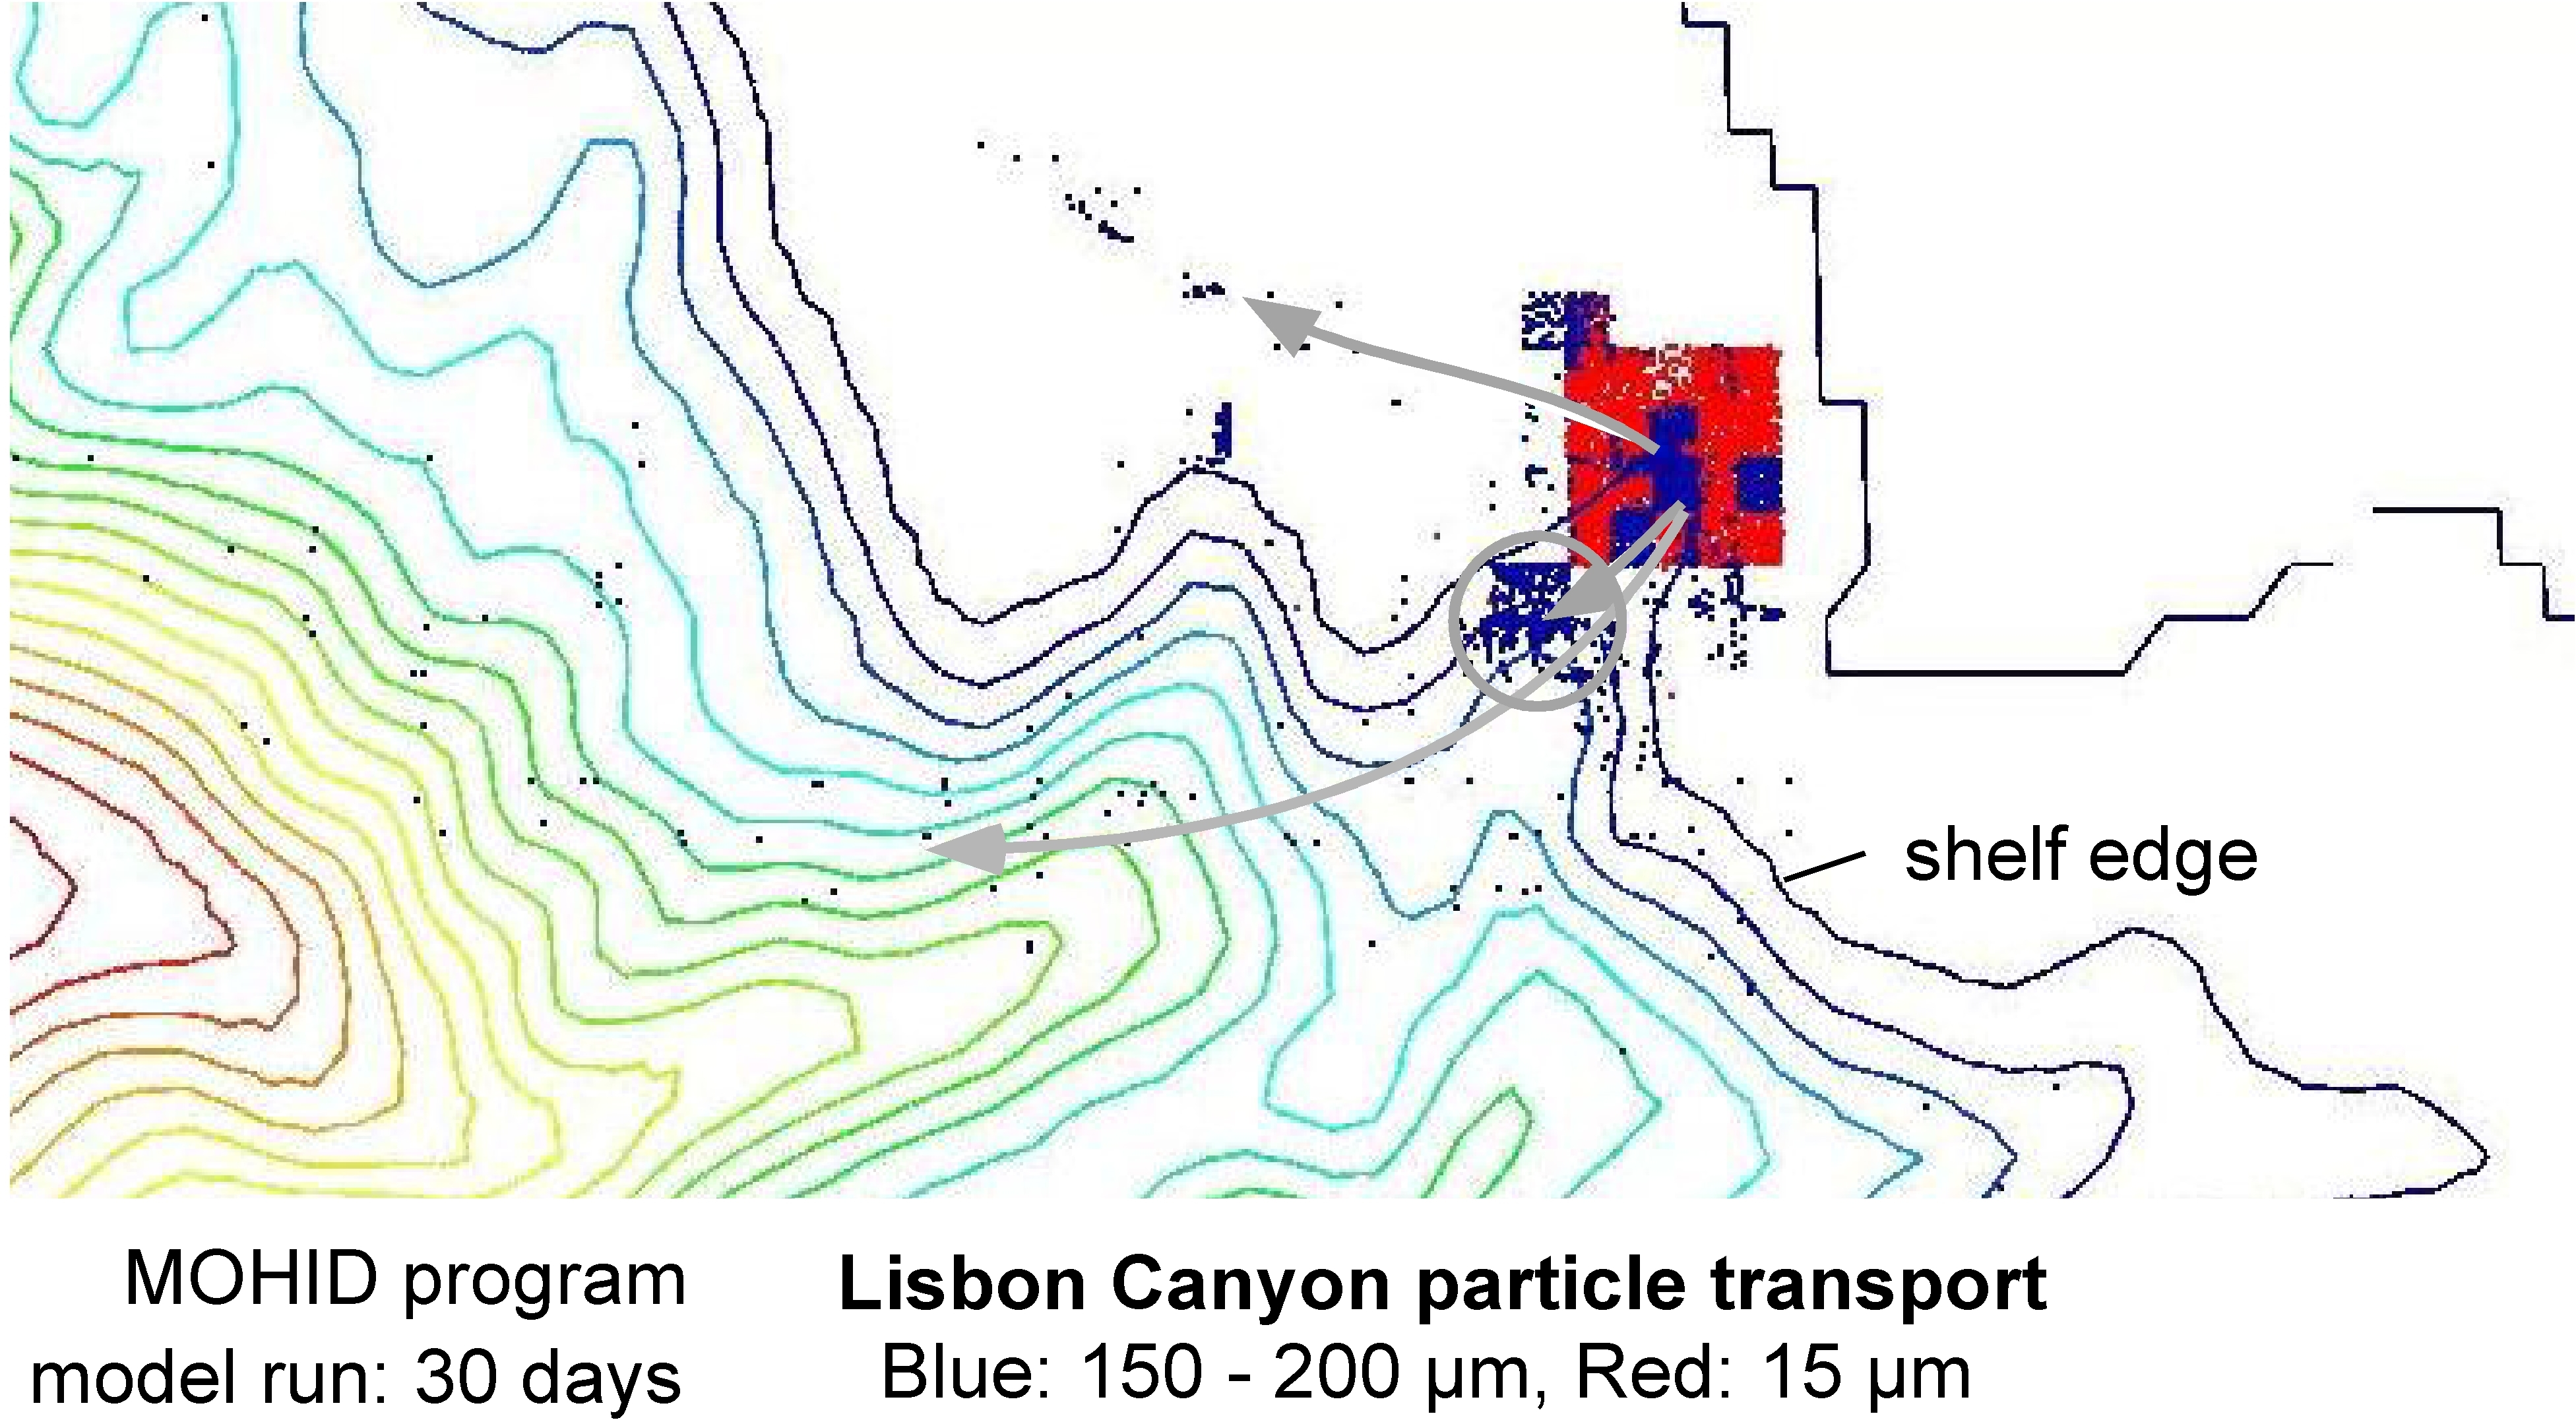
\includegraphics[width=\hsize]{Thomsen/LisboaModel.jpg}
%        
\includegraphics[width=6cm]{sample.jpg}
    \mycaption{ Results from model run on the transfer from the
    canyon head of  fine sediments (red) and organo-mineral-aggregates
    (blue) within Lisbon Canyon after a period of 30 days.)}\label{fig:Thomsen_2006_Fig}
   \end{center}
\end{figure}


{\it NEPTUNE:} Another research highlight were first studies
with internet operated vehicles in the Baltic, the ''Seep Finder''
and the ''Micro-Profiler'' (in collaboration MPI Bremen). The
IRCCM/Statoil project represents one of the first observatories
with real-time data transfer to the wold wide web. The internet
operated vehicles were developed in OceanLab. The geological
settings at the project-site are comparable with those at the
planned international deep sea observatories. Like in the
US/Canadian NEPTUNE program the investigation of cold seeps, fluid
flow and gas release plays the central role. Online recorded CTD
casts and data from oxygen microprofilers revealed additional
evidence for pressure (sealevel) controlled Methane release and
hydrodynamic-controlled oxygen penetration depth.

{\it OceanGreenhouse:} The study was carried out to
investigate the prospect of developing a large scale
photosynthetic system for greenhouse gas control. The aim was to
use marine microalgae as an enhanced natural sink for carbon
dioxide emissions from an coal-fired power plant. The annual
production of marine microalgae ranged from 0.6 - 20 t/ha/month
(extrapolated). The biomass could be used as animal feed with
heavy metal contaminations of one order of magnitude lower than
officially tolerated. The percentage of total lipid concentrations
for biodiesel production was up to 27 \% and varied  with nutrient
supply and timing of harvest. The percentages of under-saturated
fatty acids ranged between 64 and 85 \% and fatty acid composition
could be controlled.

\paragraph{Activities}
% list the (research) events you have organized, if any,

\begin{enumerate}
\item HERMES Training workshop (January 2005) \item  EGU Vienna:
three oral presentations (April 2005) \item  HERMES annual meeting
(April 2005) \item  Presentation EON $CO_2$ mitigation at EON
headquarters (May) \item  Workshop at Statoil research center
(June) \item Workshop ESONET proposal (September) \item  Workshop
CORAMM proposal (October) \item  Advisory meeting Norwegian
Deepwater Monitoring (November)
\end{enumerate}

\paragraph{Collaborations}
\noindent

Regional:
\begin{enumerate}
\item {\sl E.on} \\ Dr.
Daniela Krause \\ E.on II on carbon dioxide mitigation
\item {\sl The German
Navy} \\BOOM (Baltic Ocean Observatory)
\end{enumerate}

National:
\begin{enumerate}
\item {\sl
Bluebiotech/Sacco} \\ Dr. Sebastian Lippemeier\\ Marigel II
\end{enumerate}

International:
\begin{enumerate}
\item {\sl University of Victoria, Canada} \\ Prof. Ross Chapman \\
NEPTUNE Canada (North-East Pacific Time-series Undersea Network Experiments
 \item {\sl University of Washington, USA} \\ Prof. John Delaney \\
NEPTUNE USA
\item {\sl 34 other EU institutions} \\ Prof. Phil Weaver \\
HERMES (Hotspot Ecosystem Research on the Margins of European
Seas) \item {\sl 25 other EU Institutions} \\ Dr. Fran\c{c}ois
Rolin \\ ESONET (European Seafloor Observatory Network) \item
{\sl4 other EU institutions} \\ Dr. Thomas Lundalv \\ CORAMM,
(COral Risk Assessment Monitoring and Modeling) \item {\sl
Monterey Bay Research Institute (USA)} \\ Prof. Marsha McNutt \\
MARS (Monterey Accelerated Research System)   \item
{\sl Statoil, Norway} \\ Prof. Per Arne Bjorkum \\ Ocean
observatory \item {\sl University of Washington, USA} \\ Prof.
Jody Deming  \\ IGERT
\end{enumerate}


\paragraph{Grants}
% list the running grants in 2005, if none have been received, please delete this
% subsection.
\begin{enumerate}

\item
Funded by EU, \emph{Esonet II}, WP leader, P.I., (2006 - )

\item
Funded by EU, \emph{HERMES}, WP leader, P.I., (April 2005 -  March 2009)

\item
\emph{Neptune Canada},  P.I., CA, (April 2006 - April 2007)

\item
Funded by private industry, \emph{IRCCM observatory}, coordinator, EU/US, (January 2006 -
December 2008) 

\item
Funded by E.on, \emph{carbon mitigation II}, coordinator, D, (August 2005 - September
2006) 

\item
Funded by Private Industry Statoil, \emph{CORAMM}, coordinator, (October 2006 - May 2010) 
\end{enumerate}

\paragraph{Other Support Grants}
\begin{enumerate}
\item IGERT: exchange program Seattle-Bremen
\item BOOM: P.I., D 2005-2008
 \item OceanGreenhouse: coordinator,
D 2005-
\end{enumerate}


\nocite{Thomsen1} \nocite{Thomsen2} \nocite{Thomsen3}
\nocite{Thomsen4} \nocite{Thomsen5}
